\chapter{Ước lượng chiếu và lựa chọn mô hình}\label{ch:projection}
\section{Bắt đầu bằng ba câu hỏi, chưa cần toán cao cấp}
Bạn đã gặp histogram ở Chương 2: chia miền thành các ô, đếm dữ liệu,
rồi vẽ một chiều cao trên mỗi ô. Ước lượng chiếu mở rộng ý tưởng này:
\emph{chọn một số hình dạng đơn giản, rồi ghép chúng thành đường ước lượng}.

Trong chương này, ta trả lời lần lượt ba câu hỏi:
\begin{enumerate}
\item \textbf{Ghép bằng cái gì?} Dùng các hàm cơ sở: có thể là hình chữ
nhật, hoặc sóng sin và cos.
\item \textbf{Mỗi hình dạng đóng góp bao nhiêu?} Tính các hệ số từ dữ liệu.
\item \textbf{Dùng bao nhiêu hình dạng?} Chọn số chiều $D$: ít quá thì
mất chi tiết, nhiều quá thì giữ cả nhiễu của mẫu.
\end{enumerate}
\textbf{Cách đọc.} Lần đầu, đọc từ ví dụ histogram đến phần oracle và câu
hỏi tự kiểm tra. Phần ``Đọc thêm'' ở cuối giữ các chứng minh nâng cao;
bạn có thể quay lại sau khi giải thích được ví dụ bằng lời.
Không cần hiểu chuỗi vô hạn ngay để tính được một ước lượng chiếu.

\intuition{Hãy coi $D$ là số thành phần bạn cho phép đường ước lượng sử
 dụng. Bài toán có hai bước riêng: với $D$ đã cho, dựng đường; sau đó mới
 so sánh các $D$ để chọn đường phù hợp.}

\section{Một ví dụ histogram dùng xuyên suốt chương}
\subsection{Dữ liệu và ba cách chia ô}
Giả sử dữ liệu nằm trên $[0,1]$. Cho tám quan sát
\[
X=(0.10,0.12,0.20,0.30,0.40,0.60,0.80,0.90),\qquad n=8.
\]
Ta thử $D=1,2,4$ ô bằng nhau. Độ rộng mỗi ô là $h=1/D$.
Chiều cao mật độ trong một ô luôn là
\[
\boxed{\text{chiều cao}=\frac{\text{số điểm trong ô}}{n\times h}.}
\]
\begin{center}
\begin{tabular}{cccc}
\toprule Số ô $D$ & Độ rộng $h$ & Số đếm trong các ô & Chiều cao mật độ\\\midrule
1 & $1$ & $(8)$ & $(1)$\\
2 & $1/2$ & $(5,3)$ & $(5/4,3/4)$\\
4 & $1/4$ & $(3,2,1,2)$ & $(3/2,1,1/2,1)$\\\bottomrule
\end{tabular}
\end{center}
Ví dụ, với $D=2$, ô trái có năm điểm nên chiều cao là
$5/(8\times1/2)=5/4$. Ô phải có ba điểm nên chiều cao là $3/4$.
Diện tích hai ô là $5/4\times1/2+3/4\times1/2=1$.

\subsection{Tại sao đây đã là một bài toán chọn mô hình?}
Với một ô, đường chỉ có một mức cao nên không thể hiện sự khác nhau giữa
hai nửa miền. Với bốn ô, đường có thể hiện nhiều chi tiết hơn; nhưng chỉ
một điểm đi sang ô kế bên cũng có thể làm chiều cao đổi đáng kể.
Cả ba đường đều được dựng từ cùng tám điểm. \emph{Nhiều ô hơn không tự
động có nghĩa gần mật độ thật hơn.} Ta chưa biết mật độ thật để chấm sai
số trực tiếp; đó là lý do cần tiêu chuẩn lựa chọn mô hình.

\begin{figure}[htbp]
\centering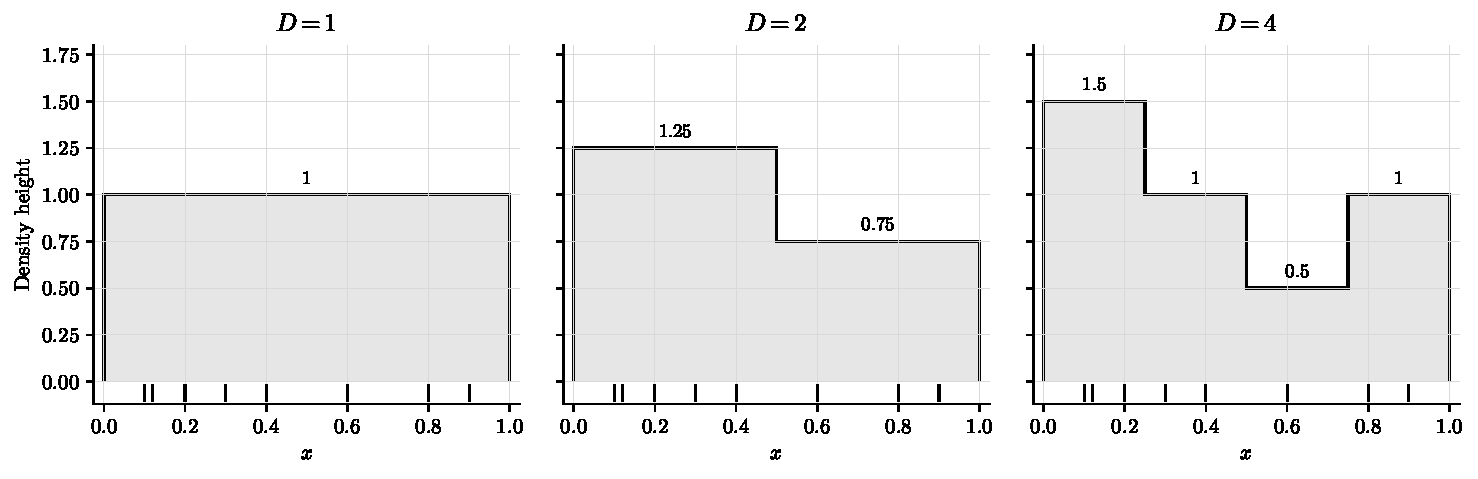
\includegraphics[width=.97\textwidth]{projection_models.pdf}
\caption{Cùng tám quan sát, ba mô hình histogram với $D=1,2,4$.
Các vạch dưới trục là dữ liệu. Chiều cao từng ô được tính trong bảng;
không có đường mật độ thật trong hình vì ví dụ chỉ cho dữ liệu.}
\end{figure}
\intuition{Ở ví dụ hàm bước, ``mô hình $D$ chiều'' chỉ là tập các đường
có một chiều cao trên mỗi ô. Chọn mô hình nghĩa là chọn mức độ chi tiết.}

\section{Hàm cơ sở và hệ số: đọc như một công thức ghép hình}
\subsection{Trước tiên, dùng hai hình chữ nhật}
Với $D=2$, đặt $B_1=[0,1/2)$, $B_2=[1/2,1]$.
Một hàm chỉ báo $\1_{B_j}(x)$ bằng 1 khi $x$ trong ô $j$, bằng 0 ở ngoài.
Ta có thể viết histogram thành
\[
\widehat f_2(x)=\frac54\1_{B_1}(x)+\frac34\1_{B_2}(x).
\]
Dòng này chỉ nói: ở ô trái, lấy chiều cao $5/4$; ở ô phải, lấy $3/4$.
Các hình chữ nhật là \emph{hàm cơ sở}; các số đứng trước chúng là
\emph{hệ số}. Với cơ sở tổng quát, hệ số không nhất thiết là chiều cao
hay xác suất của một ô.

\subsection{Tại sao trong slide lại có căn bậc hai?}
Để phép tính gọn hơn, ta dùng các hàm cơ sở được chuẩn hóa:
\[
\phi_1(x)=\sqrt2\,\1_{B_1}(x),\qquad
\phi_2(x)=\sqrt2\,\1_{B_2}(x).
\]
Mỗi hình chữ nhật cao $\sqrt2$, rộng $1/2$. Vì vậy tích phân
\emph{bình phương} của mỗi hàm bằng
$(\sqrt2)^2\times1/2=1$.
Hai hàm không chồng lên nhau, nên tích của chúng bằng 0 tại mọi điểm.
Ta gọi hai tính chất này là \emph{trực chuẩn}:
\[
\int_0^1\phi_1^2=\int_0^1\phi_2^2=1,\qquad
\int_0^1\phi_1\phi_2=0.
\]
``Chuẩn'' nghĩa là độ lớn đã đưa về 1; ``trực'' nghĩa là hai hình dạng
không có phần tích chung khi lấy tích phân. Với sin và cos, các hàm có
thể chồng lên nhau nhưng các phần dương và âm của tích triệt tiêu.

\subsection{Tính hệ số từ mẫu, rồi ghép lại}
Công thức hệ số mẫu là trung bình các giá trị hàm cơ sở tại dữ liệu:
\[
\widehat a_j=\frac1n\sum_{i=1}^n\phi_j(X_i).
\]
Ở ví dụ hai ô, $\phi_1(X_i)$ bằng $\sqrt2$ ở năm điểm, bằng 0 ở ba
điểm. Do đó
\[
\widehat a_1=\frac{5\sqrt2}{8},\qquad
\widehat a_2=\frac{3\sqrt2}{8}.
\]
Ghép hai hình dạng:
\begin{align*}
\widehat f_2(x)
&=\widehat a_1\phi_1(x)+\widehat a_2\phi_2(x)\\
&=\frac{5\sqrt2}{8}\sqrt2\,\1_{B_1}(x)
 +\frac{3\sqrt2}{8}\sqrt2\,\1_{B_2}(x)\\
&=\frac54\1_{B_1}(x)+\frac34\1_{B_2}(x).
\end{align*}
Hai căn nhân nhau thành 2, nên kết quả trùng histogram ban đầu.
\textbf{Bạn chưa học một estimator khác: bạn vừa viết lại histogram
bằng ngôn ngữ hàm cơ sở.}

Với $D$ ô, mỗi ô rộng $1/D$, cơ sở chuẩn hóa cao $\sqrt D$:
\[
\phi_{D,j}=\sqrt D\,\1_{B_j},\qquad
\widehat a_{D,j}=\frac{\sqrt D N_j}{n},\qquad
\widehat f_D(x)=\frac{DN_j}{n}\quad(x\in B_j).
\]
Chỉ số $D,j$ nhắc rằng cơ sở hàm bước thay đổi khi đổi phân hoạch.
\intuition{Hàm cơ sở cho hình dạng; hệ số cho mức đóng góp. Căn bậc hai
là cách chuẩn hóa để phép tính bình phương đơn giản, không phải một thao
 tác bí ẩn trên dữ liệu.}
\source{\cite{projection}, slide 8--12; \cite{slide2}, slide 30--31}

\section{Phân biệt ba đường: thật, xấp xỉ và ước lượng}
Đây là ba ký hiệu dễ nhầm nhất trong chương:
\begin{center}
\begin{tabular}{p{.12\textwidth}p{.39\textwidth}p{.37\textwidth}}
\toprule Ký hiệu & Đọc bằng lời & Ta có tính từ dữ liệu không?\\\midrule
$f$ & Mật độ thật cần tìm & Không, nói chung chưa biết.\\[3pt]
$f_D$ & Đường gần $f$ nhất trong mô hình $D$ đã chọn & Không, cần biết $f$.\\[3pt]
$\widehat f_D$ & Đường ta dựng từ mẫu, trong mô hình $D$ & Có.\\\bottomrule
\end{tabular}
\end{center}
Dấu mũ có nghĩa là dùng dữ liệu để ước lượng. $f_D$ không có dấu mũ vì
nó là một đối tượng lý thuyết, không phải kết quả tính từ mẫu.

Với một cơ sở trực chuẩn, hệ số thật và hệ số mẫu là
\[
a_j=\int_0^1\phi_j(x)f(x)\,dx=\E\phi_j(X),\qquad
\widehat a_j=\frac1n\sum_i\phi_j(X_i).
\]
Công thức bên trái lấy trung bình theo phân phối thật, bên phải lấy
trung bình tám giá trị quan sát. Đó là nguyên lý thế của Chương 1.
\[
\boxed{f_D=\sum_{j=1}^D a_j\phi_j,\qquad
\widehat f_D=\sum_{j=1}^D\widehat a_j\phi_j.}
\]
Vì trung bình mẫu có kỳ vọng bằng trung bình thật,
$\E\widehat a_j=a_j$ và $\E\widehat f_D=f_D$.
Nhưng $f_D$ có thể khác $f$: mô hình quá đơn giản vẫn làm mất chi tiết,
ngay cả khi các hệ số được tính chính xác.

\subsection{Vì sao gọi là ``chiếu''?}
Hãy nghĩ đến việc biểu diễn một vật bằng cái bóng của nó trên một mặt
phẳng. Cái bóng chỉ giữ phần thông tin biểu diễn được trên mặt phẳng ấy.
Tương tự, $f_D$ chỉ giữ những hình dạng nằm trong mô hình đã chọn.

Tên chính thức của mô hình là $S_D$, tức tập các tổng
$g=\sum_{j=1}^Db_j\phi_j$ khi các hệ số $b_j$ được phép thay đổi.
Từ ``span'' trong slide chỉ chính tập những tổng đó.
Phép chiếu chọn tổng gần $f$ nhất theo sai số bình phương tích phân;
khái niệm gần sẽ được tính cụ thể ngay dưới đây.
\intuition{Có hai nguyên nhân gây sai: mô hình chưa đủ biểu diễn đường
thật, và mẫu hữu hạn làm các hệ số bị lệch khỏi giá trị thật. Đừng gộp
$f_D$ và $\widehat f_D$ thành một đường.}

\section{Đo sai số và hiểu Pythagoras bằng một ví dụ}
\subsection{Chuẩn L2 chỉ là tích phân sai khác bình phương}
Ký hiệu trong slide
\[
\norm{g-f}_2^2=\int_0^1[g(x)-f(x)]^2\,dx
\]
được đọc như sau: tại mỗi vị trí, lấy chênh lệch hai chiều cao; bình phương
để sai khác âm không bù sai khác dương; cộng liên tục trên toàn miền
bằng tích phân. Giá trị càng nhỏ thì hai đường càng gần theo tiêu chí này.
$L_2$ là tên của không gian các hàm có tích phân bình phương hữu hạn;
trong phần tính bài, hãy nhớ công thức tích phân ở trên.

Nếu hai đường hằng trên cùng các ô, không cần tích phân khó:
\[
\text{sai số}=\sum_j(\text{chênh lệch chiều cao ở ô }j)^2
 \times\text{độ rộng ô }j.
\]
Còn ký hiệu $\inner gq=\int_0^1g(x)q(x)dx$ được gọi là tích vô hướng.
Nó giúp kiểm tra các phần sai số có trực giao hay không.

\subsection{Ví dụ với một mật độ thật được cho để luyện tính}
Riêng mục này, giả sử \emph{đề cho} $f(x)=2x$ trên $[0,1]$.
Với hai ô, đường tốt nhất hằng trên mỗi ô lấy chiều cao trung bình thật:
\[
f_2(x)=\begin{cases}1/2,&0\leq x<1/2,\\3/2,&1/2\leq x\leq1.
\end{cases}
\]
Chẳng hạn chiều cao ô trái là
$(1/(1/2))\int_0^{1/2}2x\,dx=2(1/4)=1/2$.
Trong khi đó mẫu tám điểm phía trên cho chiều cao $(5/4,3/4)$ của
$\widehat f_2$. Mẫu nhỏ này không nhất thiết đại diện tốt cho $f$ đã cho.

\step{Sai số thứ nhất: mô hình làm mất độ dốc.}
Đường $f_2$ hằng trong ô, còn $f$ tăng. Tính được
\[
\int_0^{1/2}(2x-1/2)^2dx+
\int_{1/2}^1(2x-3/2)^2dx=\frac1{12}.
\]
Để tự kiểm tra, nguyên hàm của $(2x-c)^2$ là
$4x^3/3-2cx^2+c^2x$; dùng $c=1/2$ hoặc $3/2$ ở từng ô.

\step{Sai số thứ hai: hệ số tính từ mẫu khác hệ số thật.}
Trong hai ô, chênh lệch chiều cao giữa $\widehat f_2$ và $f_2$ là
$3/4$ và $-3/4$. Do đó
\[
\norm{\widehat f_2-f_2}_2^2
=(3/4)^2(1/2)+(-3/4)^2(1/2)=\frac9{16}.
\]
\step{Tổng sai số.}
Tính trực tiếp từ đường thật đến đường ước lượng cho
\[
\norm{f-\widehat f_2}_2^2=
\int_0^{1/2}(2x-5/4)^2dx+
\int_{1/2}^1(2x-3/4)^2dx
=\frac{31}{48}=\frac1{12}+\frac9{16}.
\]
Đây là sai số của mẫu cụ thể này, không phải kỳ vọng qua mọi mẫu.

\subsection{Chứng minh vì sao hai phần cộng được}
Đặt $e_1=f-f_D$, $e_2=f_D-\widehat f_D$. Khi đó
$f-\widehat f_D=e_1+e_2$.
Khai triển bình phương như với hai số thông thường:
\[
\int(e_1+e_2)^2=\int e_1^2+\int e_2^2+2\int e_1e_2.
\]
Với histogram, $e_2$ hằng trong mỗi ô, còn
$\int_{B_j}(f-f_D)=0$ vì $f_D$ là trung bình ô.
Do đó trên mỗi ô, hằng số $e_2$ nhân tích phân bằng 0:
$\int_{B_j}e_1e_2=e_2|_{B_j}\int_{B_j}e_1=0$.
Cộng các ô cho hạng chéo bằng 0.

Với cơ sở trực chuẩn tổng quát, lý do tương tự:
$\inner{f-f_D}{\phi_j}=a_j-a_j=0$ cho $j\leq D$, trong khi $e_2$ là
một tổng các $\phi_j$ đó. Vì vậy $\inner{e_1}{e_2}=0$ và
\[
\boxed{\underbrace{\norm{f-\widehat f_D}_2^2}_{\text{tổng sai số}}
=\underbrace{\norm{f-f_D}_2^2}_{\text{sai do mô hình}}
+\underbrace{\norm{f_D-\widehat f_D}_2^2}_{\text{sai do mẫu}}.}
\]
Đây là Pythagoras trong không gian hàm. Hạng chéo mất do trực giao,
không phải vì các hệ số độc lập.

\subsection{Bias--variance đọc bằng lời}
Lấy trung bình tổng sai số qua nhiều mẫu mới được rủi ro:
\[
\E\norm{f-\widehat f_D}_2^2
=\norm{f-f_D}_2^2+\E\norm{f_D-\widehat f_D}_2^2.
\]
Phần đầu không đổi khi lấy mẫu lại: đó là bình phương bias tích phân.
Phần sau dao động theo mẫu: kỳ vọng của nó là tổng variance của các hệ số.
\intuition{Bạn có thể biết chính xác mật độ nhưng vẫn không vẽ được độ
 dốc bằng một ô hằng; đó là giới hạn mô hình. Ngược lại, dù đã chọn mô
 hình tốt, ít dữ liệu vẫn làm chiều cao ước lượng thiếu ổn định.}
\source{\cite{projection}, slide 13--15; \cite{slide2}, slide 32}

\section{Contrast: một điểm số tính được khi không biết mật độ thật}
\subsection{Vì sao phải tạo điểm số khác?}
Ta muốn chấm $\int(g-f)^2$, nhưng không biết $f$.
Khai triển:
\[
\int(g-f)^2=\int g^2-2\int gf+\int f^2.
\]
Hạng cuối giống nhau cho tất cả đường $g$, nên bỏ nó không đổi thứ tự
so sánh. Với hai điểm số $A+c$ và $B+c$, so sánh vẫn như $A$ với $B$.
Hạng $\int gf$ là kỳ vọng $\E g(X)$, được ước lượng bằng trung bình mẫu.
Do đó định nghĩa
\[
\boxed{\gamma_n(g)=\int_0^1g(x)^2dx-
\frac2n\sum_{i=1}^ng(X_i).}
\]
Chữ $\gamma_n$ là tên điểm số, gọi là \emph{contrast} hay hàm tương phản.
Nó có thể âm; không phải chính sai số bình phương.
Với $g$ cố định trước khi nhìn mẫu,
$\E\gamma_n(g)=\norm{g-f}_2^2-\norm f_2^2$.
Nếu $g$ được chọn từ chính mẫu, không tự áp dụng đẳng thức này như thể
$g$ cố định; bước chọn mô hình cần kiểm soát riêng.

\subsection{Tại sao cực tiểu contrast cho đúng hệ số mẫu?}
Đặt $g=\sum_{j=1}^Db_j\phi_j$; $b_j$ là những hệ số ta đang thử.
Trực chuẩn làm $\int g^2=\sum_jb_j^2$.
Trung bình mẫu của $g$ là
\[
\frac1n\sum_i g(X_i)
=\sum_j b_j\left(\frac1n\sum_i\phi_j(X_i)\right)
=\sum_jb_j\widehat a_j.
\]
Vậy
\begin{align*}
\gamma_n(g)&=\sum_j(b_j^2-2b_j\widehat a_j)\\
&=\sum_j\{(b_j-\widehat a_j)^2-\widehat a_j^2\}.
\end{align*}
Ở dòng cuối dùng $(b-a)^2=b^2-2ba+a^2$.
Các $\widehat a_j$ đã tính được từ mẫu nên là hằng khi ta thay đổi $b_j$.
Để điểm số nhỏ nhất, chỉ cần làm mọi $(b_j-\widehat a_j)^2$ bằng 0:
chọn $b_j=\widehat a_j$.
\[
\boxed{\text{Đường có contrast nhỏ nhất trong }S_D\text{ là }
\widehat f_D.}
\]
Không cần đạo hàm hay nghịch đảo ma trận để hiểu kết luận này.
Thế các hệ số tối ưu lại cho
\[
\gamma_n(\widehat f_D)=-\sum_j\widehat a_j^2
=-\norm{\widehat f_D}_2^2.
\]
\intuition{Contrast là cách dùng mẫu thay phần không biết trong công
 thức sai số. Với mỗi mô hình đã cho, hoàn thành bình phương giải thích
 ngay vì sao ta lấy trung bình mẫu làm hệ số.}
\source{\cite{projection}, slide 12; \cite{slide2}, slide 33}

\section{Lựa chọn mô hình: tính điểm rồi cộng phạt}
\subsection{Vì sao contrast chưa đủ?}
Khi các mô hình lồng nhau, thêm thành phần có thể làm
$\sum_j\widehat a_j^2$ tăng, nên điểm số âm
$-\sum_j\widehat a_j^2$ giảm. Chỉ lấy contrast nhỏ nhất dễ luôn ưu tiên
mô hình lớn, kể cả khi thành phần mới chủ yếu là nhiễu.

Ta thêm một khoản phạt tăng theo số chiều:
\[
\text{điểm chọn mô hình}=
\underbrace{-\norm{\widehat f_D}_2^2}_{\text{contrast}}
+\underbrace{\kappa\phi_0D/n}_{\text{phạt độ phức tạp}}.
\]
$\kappa$ quyết định phạt mạnh hay nhẹ. $\phi_0$ là một hằng số kiểm soát
độ lớn cơ sở; với histogram chia đều, dùng $\phi_0=1$.
Ý nghĩa quan trọng trước tiên: mô hình lớn phải cải thiện contrast đủ
nhiều để bù khoản phạt thêm.

\subsection{Tính tất cả điểm số trên mẫu tám quan sát}
Với hàm hằng theo ô, $\norm{\widehat f_D}_2^2$ bằng tổng
\emph{chiều cao bình phương nhân độ rộng}. Từ bảng đầu chương:
\begin{align*}
D=1:\quad&1^2\times1=1,\\
D=2:\quad&(5/4)^2(1/2)+(3/4)^2(1/2)=17/16,\\
D=4:\quad&[(3/2)^2+1^2+(1/2)^2+1^2]/4=9/8.
\end{align*}
\emph{Riêng bài tính này}, cho $\kappa=1/3$, $\phi_0=1$, $n=8$.
Penalty bằng $D/24$; không cần tự tìm $\kappa$.
\begin{center}
\begin{tabular}{cccc}
\toprule $D$ & Contrast & Phạt $D/24$ & Tổng điểm\\\midrule
1 & $-1$ & $1/24$ & $-23/24\approx-0.95833$\\
2 & $-17/16$ & $1/12$ & $-47/48\approx-0.97917$\\
4 & $-9/8$ & $1/6$ & $-23/24\approx-0.95833$\\\bottomrule
\end{tabular}
\end{center}
Số nhỏ nhất là $-47/48$, nên chọn $\boxed{\widehat D=2}$ và dùng
histogram hai ô. Nếu bỏ khoản phạt, $D=4$ có contrast nhỏ nhất.
Ví dụ minh họa phép tính điểm; không khẳng định $\kappa=1/3$ là hệ số
đủ cho định lý oracle hoặc hai ô chắc chắn tốt nhất với mật độ thật.

\subsection{Giải mã công thức trên slide}
\[
\boxed{\widehat D\in\argmin_{D\in\mathcal D_n}
\{-\norm{\widehat f_D}_2^2+\operatorname{pen}(D)\}.}
\]
Đọc từng phần: $\mathcal D_n$ là danh sách số chiều ứng viên, ở ví dụ là
$\{1,2,4\}$; $\operatorname{pen}(D)$ là khoản phạt;
$\argmin$ nghĩa là \emph{lấy giá trị $D$ làm điểm số nhỏ nhất}, không
phải lấy chính điểm số nhỏ nhất. Ví dụ $\argmin$ trả về 2, còn điểm nhỏ
nhất là $-47/48$. Nếu nhiều $D$ bằng điểm, chọn $D$ nhỏ hơn.

Một mô hình gọi là \emph{lồng nhau} khi mọi đường của mô hình nhỏ cũng
biểu diễn được trong mô hình lớn. Histogram một ô nằm trong mô hình hai
ô: chỉ cần hai chiều cao bằng nhau. Mô hình hai ô nằm trong mô hình bốn
ô: mỗi ô cũ được chia đôi, dùng cùng chiều cao trên hai ô mới.
Vì vậy $D=1,2,4,8,\ldots$ cho mô hình lồng nhau. Các phân hoạch
$D=2$ và $D=3$ nói chung không có tính chất ấy.
\intuition{Chọn mô hình là so sánh lợi ích của thêm chi tiết với giá phải
 trả do thêm nhiễu. Penalty lớn hơn thường thiên về mô hình đơn giản hơn.
 Đừng học thuộc $\argmin$ trước khi tự tính được bảng điểm.}
\source{\cite{projection}, slide 20--23; \cite{slide2}, slide 33}

\section{Oracle và thích nghi: hiểu lời hứa của định lý}
\subsection{Oracle là người so sánh tưởng tượng biết mật độ thật}
Nếu biết $f$, ta có thể chọn $D$ dựa trên
\[
\underbrace{\norm{f-f_D}_2^2}_{\text{mất chi tiết}}
+\underbrace{\phi_0D/n}_{\text{chặn trên cho nhiễu lấy mẫu}}.
\]
Người tưởng tượng biết $f$ để chọn như vậy được gọi là \emph{oracle}.
Ta không có người này; oracle chỉ là chuẩn so sánh tốt nhất trong
\emph{họ mô hình đang xét}. Nó không có nghĩa biết mọi điều hay tìm
được estimator tốt nhất trong tất cả phương pháp có thể có.

\subsection{Bất đẳng thức oracle nói gì bằng lời?}
Trong những điều kiện phù hợp, định lý nói:
\begin{quote}
Sai số trung bình của cách chọn bằng dữ liệu không vượt quá một bội
của mức tốt nhất mà oracle chọn được, cộng một phần dư nhỏ.
\end{quote}
Công thức là
\[
\E\norm{\widehat f_{\widehat D}-f}_2^2
\leq C\inf_{D\in\mathcal D_n}
\left\{\norm{f-f_D}_2^2+\frac{\phi_0D}{n}\right\}+\frac{C'}n.
\]
\begin{itemize}
\item Vế trái: lấy mẫu, tự chọn $D$, dựng đường, tính sai số; rồi lấy
trung bình qua các mẫu.
\item $\inf_D$: mức tốt nhất trong các ứng viên; với danh sách hữu hạn
của ví dụ, đây là giá trị nhỏ nhất.
\item $C$: một hệ số cho phép cách chọn thực tế kém hơn oracle một mức.
Không tự hiểu $C=1$ hoặc gần 1.
\item $C'/n$: phần dư giảm khi cỡ mẫu tăng; với $C'$ cố định, tăng
$n$ gấp đôi làm phần dư này giảm một nửa.
\end{itemize}
Định lý nói về \emph{sai số trung bình}, không hứa chọn đúng mô hình
oracle trên từng mẫu. Nó cần giả thiết về mật độ, cơ sở, họ mô hình và
penalty đủ lớn tương ứng. Không dùng bất kỳ $\kappa>0$ rồi tự tuyên bố
có bảo đảm. Phần chứng minh xác suất được giữ ở mục đọc thêm.

\subsection{Thích nghi nghĩa là tự điều chỉnh mức chi tiết}
Một mật độ khá đơn giản có thể chỉ cần ít thành phần. Mật độ nhiều chi
 tiết có thể cần nhiều thành phần hơn. Ta chưa biết độ trơn của mật độ
thật, nhưng muốn cùng một quy tắc chọn mô hình hoạt động tốt trong
nhiều lớp độ trơn.
Nếu định lý oracle và điều kiện xấp xỉ của các lớp ấy thỏa, việc tự
chọn $\widehat D$ có thể đạt tốc độ rủi ro phù hợp với độ trơn thật mà
không nhập độ trơn vào quy tắc. Đó là \emph{thích nghi}.
Ở lần đọc đầu, chưa cần nhớ số mũ tiệm cận; hãy nhớ đây là bảo đảm
về khả năng tự chọn mức chi tiết dưới các giả thiết của định lý.
\intuition{Oracle cho một chuẩn để đánh giá cách chọn từ dữ liệu.
Thích nghi nói rằng quy tắc có thể tự điều chỉnh mức chi tiết khi chưa
 biết độ trơn; không nói rằng mẫu nào cũng nhận ra cấu trúc thật chính xác.}
\source{\cite{projection}, slide 23--24; \cite{slide2}, slide 34}

\section{Năm câu tự kiểm tra trước khi đọc chứng minh sâu}
\begin{enumerate}
\item \textbf{$D$ là gì?} Số thành phần cơ sở được dùng; với histogram
chia đều, đó là số ô.
\item \textbf{Dấu mũ trong $\widehat f_D$ nhắc gì?} Đường tính từ mẫu;
khác $f_D$, là đường chiếu lý thuyết của mật độ thật.
\item \textbf{Tại sao có hai phần sai số?} Mô hình mất chi tiết, và mẫu
làm hệ số bị nhiễu. Pythagoras tách đúng hai phần nhờ trực giao.
\item \textbf{$\argmin$ trả về gì?} Số chiều có điểm tốt nhất, không
phải giá trị điểm số. Trong bảng trên trả về 2.
\item \textbf{Vì sao cộng phạt?} Để thành phần thêm vào phải cải thiện
contrast đủ nhiều, tránh luôn thưởng cho mô hình lớn.
\end{enumerate}
\textbf{Bài thử ngắn.} Với mẫu tám điểm và $D=4$, hãy tính chiều cao ô
$[1/2,3/4)$. Có một điểm $0.60$, nên chiều cao là
$1/(8\times1/4)=1/2$. Tại $x=0.60$, chỉ một hàm cơ sở hình chữ nhật
khác 0; những hàm cơ sở khác không đóng góp.
Nếu bạn tự giải thích được các câu này, bạn đã nắm phần cốt lõi của
ước lượng chiếu và chọn mô hình. Các mục dưới đây phát triển cùng ý
 tưởng bằng ký hiệu tổng quát.

\section{Đọc thêm: chuỗi trực chuẩn và cơ sở lượng giác}
\subsection{Mở rộng từ hai hình chữ nhật sang nhiều hình dạng}
Trên $[0,1]$, giả sử $f\in L_2$ và $\{\phi_j\}_{j\geq1}$ là cơ sở
trực chuẩn đầy đủ. ``Đầy đủ'' nghĩa là với đủ nhiều thành phần, các tổng
có thể xấp xỉ mọi hàm trong không gian đang xét theo chuẩn $L_2$.
\[
f=\sum_{j=1}^{\infty}a_j\phi_j,\qquad
\int_0^1\phi_j\phi_k=\begin{cases}1,&j=k,\\0,&j\ne k.
\end{cases}
\]
Đẳng thức chuỗi hiểu theo hội tụ $L_2$, không tự theo từng điểm.
Lấy tích vô hướng với $\phi_k$ chỉ giữ lại $a_k$:
\[
a_k=\int_0^1f\phi_k=\E\phi_k(X).
\]
Giữ $D$ thành phần đầu cho $f_D$; thay $a_j$ bằng trung bình mẫu cho
$\widehat f_D$. Đây vẫn là quy trình ghép hình vừa học.

\subsection{Sin và cos cho một cách ghép khác}
\[
\phi_1(x)=1,\quad \phi_{2k}(x)=\sqrt2\cos(2\pi kx),\quad
\phi_{2k+1}(x)=\sqrt2\sin(2\pi kx),\quad k\geq1.
\]
Hàm hằng cho mức nền; các sóng cho các dạng biến thiên. Tích phân sin và
cos trên một chu kỳ bằng 0; tích phân bình phương bằng $1/2$, nên nhân
$\sqrt2$ đưa độ lớn bình phương về 1.
Các công thức tích thành tổng kiểm tra trực giao giữa tần số khác nhau.

Ví dụ, với mẫu $(0,0,1/4,1/4)$, giá trị cos ở hai vị trí là 1 và 0;
giá trị sin là 0 và 1. Do mỗi vị trí lặp hai lần,
\[
\widehat a_1=1,\qquad\widehat a_2=\widehat a_3=\sqrt2/2.
\]
Ghép lại cho
$\widehat f_3(x)=1+\cos(2\pi x)+\sin(2\pi x)$.
Đường có tích phân 1 nhưng tại $x=5/8$ bằng $1-\sqrt2<0$.
Vì vậy phép chiếu tổng quát không tự cho mật độ không âm.
Lấy phần dương rồi chuẩn hóa là một hiệu chỉnh thêm; khi ấy không giữ
nguyên mọi đẳng thức của estimator chiếu ban đầu.
\intuition{Histogram dùng hình chữ nhật; lượng giác dùng sóng. Thay cơ
sở làm thay khả năng biểu diễn, nhưng cách ước lượng hệ số vẫn là trung
bình giá trị hàm cơ sở trên các quan sát.}

\section{Đọc thêm: rủi ro và tốc độ hội tụ}
\subsection{Từ trực chuẩn đến tổng bình phương hệ số}
Với $g=\sum_jb_j\phi_j$, khai triển rồi tích phân:
\[
\norm g_2^2=\sum_{j,k}b_jb_k\int\phi_j\phi_k=\sum_jb_j^2.
\]
Các tích $j\ne k$ có tích phân 0. Áp dụng cho
$f_D-\widehat f_D=\sum_{j\leq D}(a_j-\widehat a_j)\phi_j$ và phần
chuỗi bị bỏ đi:
\[
\norm{f_D-\widehat f_D}_2^2=\sum_{j\leq D}(a_j-\widehat a_j)^2,
\qquad \norm{f-f_D}_2^2=\sum_{j>D}a_j^2.
\]
Vì $\widehat a_j$ là trung bình $n$ quan sát độc lập,
\[
\Var\widehat a_j=\frac1n\Var(\phi_j(X))
=\frac1n\left(\int\phi_j^2f-a_j^2\right).
\]
Lấy kỳ vọng trong Pythagoras cho
\[
\boxed{\E\norm{f-\widehat f_D}_2^2=
\sum_{j>D}a_j^2+\frac1n\sum_{j\leq D}\left(\int\phi_j^2f-a_j^2\right).}
\]
Độc lập giữa các quan sát cho hệ số $1/n$; trực chuẩn, chứ không phải
độc lập giữa các hệ số, loại các tích chéo.

\subsection{Vì sao chặn trên variance có dạng số chiều chia cỡ mẫu?}
Giả sử $\sup_x\sum_{j\leq D}\phi_j(x)^2\leq\phi_0D$.
Với histogram, tại mỗi điểm chỉ một hàm cao $\sqrt D$ khác 0, nên tổng
bình phương bằng $D$; vì vậy $\phi_0=1$.
Với lượng giác, mỗi hàm có bình phương không quá 2, nên có thể dùng
$\phi_0=2$. Khi đó
\begin{align*}
\frac1n\sum_j\Var(\phi_j(X))
&\leq\frac1n\sum_j\E\phi_j(X)^2\\
&=\frac1n\int\left(\sum_j\phi_j(x)^2\right)f(x)dx\\
&\leq\frac{\phi_0D}{n}\int f=\frac{\phi_0D}{n}.
\end{align*}
Đây là chặn trên, không phải variance chính xác trong mọi bài.

\subsection{Bỏ hằng số không làm đổi mô hình tốt nhất}
Trực giao của $f_D$ và $f-f_D$ cho
$\norm f_2^2=\norm{f-f_D}_2^2+\norm{f_D}_2^2$.
Vậy
\[
\norm{f-\widehat f_D}_2^2=
\norm f_2^2-\norm{f_D}_2^2+\norm{f_D-\widehat f_D}_2^2.
\]
Khi so sánh các $D$, $\norm f_2^2$ giống nhau nên bỏ được:
\[
\argmin_D\norm{f-\widehat f_D}_2^2
=\argmin_D\{-\norm{f_D}_2^2+\norm{f_D-\widehat f_D}_2^2\}.
\]
Đây là mục tiêu lý thuyết vì chứa $f_D$ chưa biết. Nếu tối ưu rủi ro,
phải lấy kỳ vọng trước khi chọn; không tự đổi thứ tự kỳ vọng và
$\argmin$.

\subsection{Độ trơn ảnh hưởng số chiều như thế nào?}
Với histogram, nếu $|f(x)-f(y)|\leq L|x-y|^\beta$,
$0<\beta\leq1$, trung bình ô cho
\[
|f(x)-f_D(x)|
\leq D\int_{B_j}L|x-u|^\beta du\leq LD^{-\beta}.
\]
Bình phương và tích phân trên miền dài 1 cho
$\norm{f-f_D}_2^2\leq L^2D^{-2\beta}$.
Không mở rộng kết luận này cho histogram với mọi $\beta>1$.
Với cơ sở lượng giác phù hợp lớp Sobolev tuần hoàn, điều kiện
$\sum_{j\geq2}j^{2\beta}a_j^2\leq L^2$ cũng cho
\[
\sum_{j>D}a_j^2\leq D^{-2\beta}\sum_{j>D}j^{2\beta}a_j^2
\leq L^2D^{-2\beta}.
\]
Cần xét điều kiện biên của lớp khi dùng cơ sở lượng giác.

Chặn rủi ro có dạng $G(D)=L^2D^{-2\beta}+\phi_0D/n$:
phần đầu giảm khi tăng $D$, phần sau tăng. Xem $D$ như biến dương để
lấy đạo hàm:
\[
G'(D)=-2\beta L^2D^{-2\beta-1}+\phi_0/n=0
\quad\Longrightarrow\quad
D_*=(2\beta L^2n/\phi_0)^{1/(2\beta+1)}.
\]
Chọn mức nguyên hoặc mức ứng viên gần đó cho
$D_*\asymp n^{1/(2\beta+1)}$, rủi ro
$O(n^{-2\beta/(2\beta+1)})$.
Thích nghi suy ra từ oracle khi họ ứng viên có mức gần $D_*$ và cơ sở
có chặn xấp xỉ phù hợp; phần dư $1/n$ có bậc nhỏ hơn tốc độ trên.
\intuition{Công thức tốc độ định lượng câu chuyện đã học: mô hình lớn
giảm mất chi tiết nhưng tăng nhiễu. Nó cần giả thiết lớp và cơ sở, không
phải kết quả tự động cho mọi mật độ.}
\source{\cite{projection}, slide 13--18; \cite{tsybakov}, Mục 1.7}

\section{Đọc thêm: phác thảo chứng minh oracle}
Mục này là phần nâng cao. Bạn có thể nắm ý nghĩa và tính tiêu chuẩn
chọn mô hình mà chưa đọc nó. Phác thảo giữ các bước đại số, còn bất đẳng
thức tập trung xác suất được viện dẫn dưới điều kiện nêu rõ.

Đặt $P g=\E g(X)=\inner gf$ và $\nu_n(g)=(P_n-P)g$.
Từ định nghĩa contrast,
\[
\gamma_n(g)=\norm{g-f}_2^2-\norm f_2^2-2\nu_n(g).
\]
Dấu trước $2\nu_n$ là \emph{âm}. Bởi cực tiểu hóa và
$f_D\in S_D$, với mọi $D$ cố định,
\begin{align*}
\gamma_n(\widehat f_{\widehat D})+\operatorname{pen}(\widehat D)
&\leq\gamma_n(\widehat f_D)+\operatorname{pen}(D)\\
&\leq\gamma_n(f_D)+\operatorname{pen}(D).
\end{align*}
Thay công thức contrast, ký hiệu
$A=\norm{\widehat f_{\widehat D}-f}_2^2$,
$B=\norm{f_D-f}_2^2$, cho
\[
A\leq B+2\nu_n(\widehat f_{\widehat D}-f_D)
+\operatorname{pen}(D)-\operatorname{pen}(\widehat D).
\]
Đặt
$Z_{D,D'}=\sup\{|\nu_n(t)|:t\in S_D+S_{D'},\norm t_2=1\}$.
Tính tuyến tính cho $|\nu_n(g)|\leq\norm g_2 Z_{D,D'}$ trên không gian
đó. Dùng $2uv\leq u^2/4+4v^2$ và
$\norm{\widehat f_{\widehat D}-f_D}_2^2\leq2A+2B$:
\[
A\leq\tfrac32B+\tfrac12A+4Z_{D,\widehat D}^2
+\operatorname{pen}(D)-\operatorname{pen}(\widehat D).
\]
Chuyển $A/2$ qua trái và nhân 2:
\[
A\leq3B+8Z_{D,\widehat D}^2
+2\operatorname{pen}(D)-2\operatorname{pen}(\widehat D).
\]
\textbf{Điều kiện tập trung được viện dẫn trong phác thảo:}
có các mức $p(D,D')$ sao cho
\[
8p(D,D')\leq\operatorname{pen}(D)+\operatorname{pen}(D'),\qquad
\sum_{D'\in\mathcal D_n}\E[Z_{D,D'}^2-p(D,D')]_+\leq C_0/n.
\]
Kiểm chứng điều kiện này cần bất đẳng thức quá trình thực nghiệm
(chẳng hạn Talagrand) và giả thiết họ mô hình; đó là phần xác suất nâng
cao được viện dẫn, không được chứng minh trong giáo trình lấy gốc.
Thế $Z^2\leq p+(Z^2-p)_+$ và bỏ số hạng phạt âm còn lại:
\[
A\leq3B+3\operatorname{pen}(D)
+8\sum_{D'}[Z_{D,D'}^2-p(D,D')]_+.
\]
Lấy kỳ vọng và infimum theo $D$ cho phiên bản oracle chặt chẽ dưới điều
kiện tập trung đã nêu:
\[
\E A\leq3\inf_D\{B+\operatorname{pen}(D)\}+8C_0/n.
\]
Nếu penalty tỷ lệ $\phi_0D/n$ với hệ số cố định đủ lớn, đây chính là
dạng oracle ở trên sau khi gộp hằng số.


\source{\cite{projection}, slide 20--24; \cite{slide2}, slide 33--34.
Dấu của đồng nhất thức contrast được kiểm tra từ định nghĩa}

\subsection{Nếu dữ liệu nằm trên một khoảng khác}
Với miền biết trước $[a,b]$, đổi $U=(X-a)/(b-a)$, ước lượng trên
$[0,1]$, rồi chuyển mật độ về đơn vị ban đầu:
\[
\widehat f_X(x)=\frac1{b-a}\widehat f_U((x-a)/(b-a)).
\]
Chiều dài mới gấp $b-a$ lần, nên chiều cao chia cho $b-a$ để diện tích
vẫn bằng 1. Hệ số $1/\sqrt{b-a}$ chỉ dành cho chuẩn hóa cơ sở $L_2$,
không thay thế hệ số đổi mật độ này.
